
% Referring to the immunity stratification as the vaccination stratification here, for the Bhutan application
History of vaccination is captured by stratifying all model compartments by vaccination status.
Two vaccination strata are included to represent those who have received at least two doses of a COVID-19 vaccine,
and those who have not.

We use data from \textit{Our World in Data} to inform the modelled dynamic vaccination coverage. In particular, we use the reported proportion of 
people ``fully vaccinated'' to specify the time-variant proportion of vaccinated people in our model. We assume that older individuals are vaccinated 
first by prioritising the modelled age groups in descending order. That is, the oldest age group receives all available vaccines until a 
saturation coverage of 80\% is reached for this group. Then the next oldest category starts receiving vaccines and we repeat this process until all available vaccines
are allocated. Note that in the event that the population-level vaccine coverage exceeds 80\%, the saturation coverage is set equal to the population-level coverage. 

Let us consider two successive time points $t_i$ and $t_{i+1}$ for which vaccination data is available. Let us denote $r_{a, i}$ and $r_{a, i+1}$ the associated vaccine 
coverage for age group $a$. The time-variant and age-specific vaccination rate per capita $w_a(t)$ verifies:

\begin{equation}
    1 - r_{a, i+1} = (1 - r_{a, i})e^{-w_a(t)(t_{i+1} - t_i)} \quad, \forall t \in [t_i, t_{i+1}) .
\end{equation}

Then, 
\begin{equation}
    \label{eq:vacc}
    w_a(t) = \frac{\ln(1 - r_{a, i}) - \ln(1 - r_{a, i+1})}{t_{i+1} - t_i} \quad, \forall t \in [t_i, t_{i+1}) ,
\end{equation}
where $\ln(x)$ represents the natural logarithm of $x$.

Figure \ref{fig:vaccination} shows the modelled vaccination coverage over time against the reported data for the analysed countries.

\begin{figure}[h]
    \begin{center}
    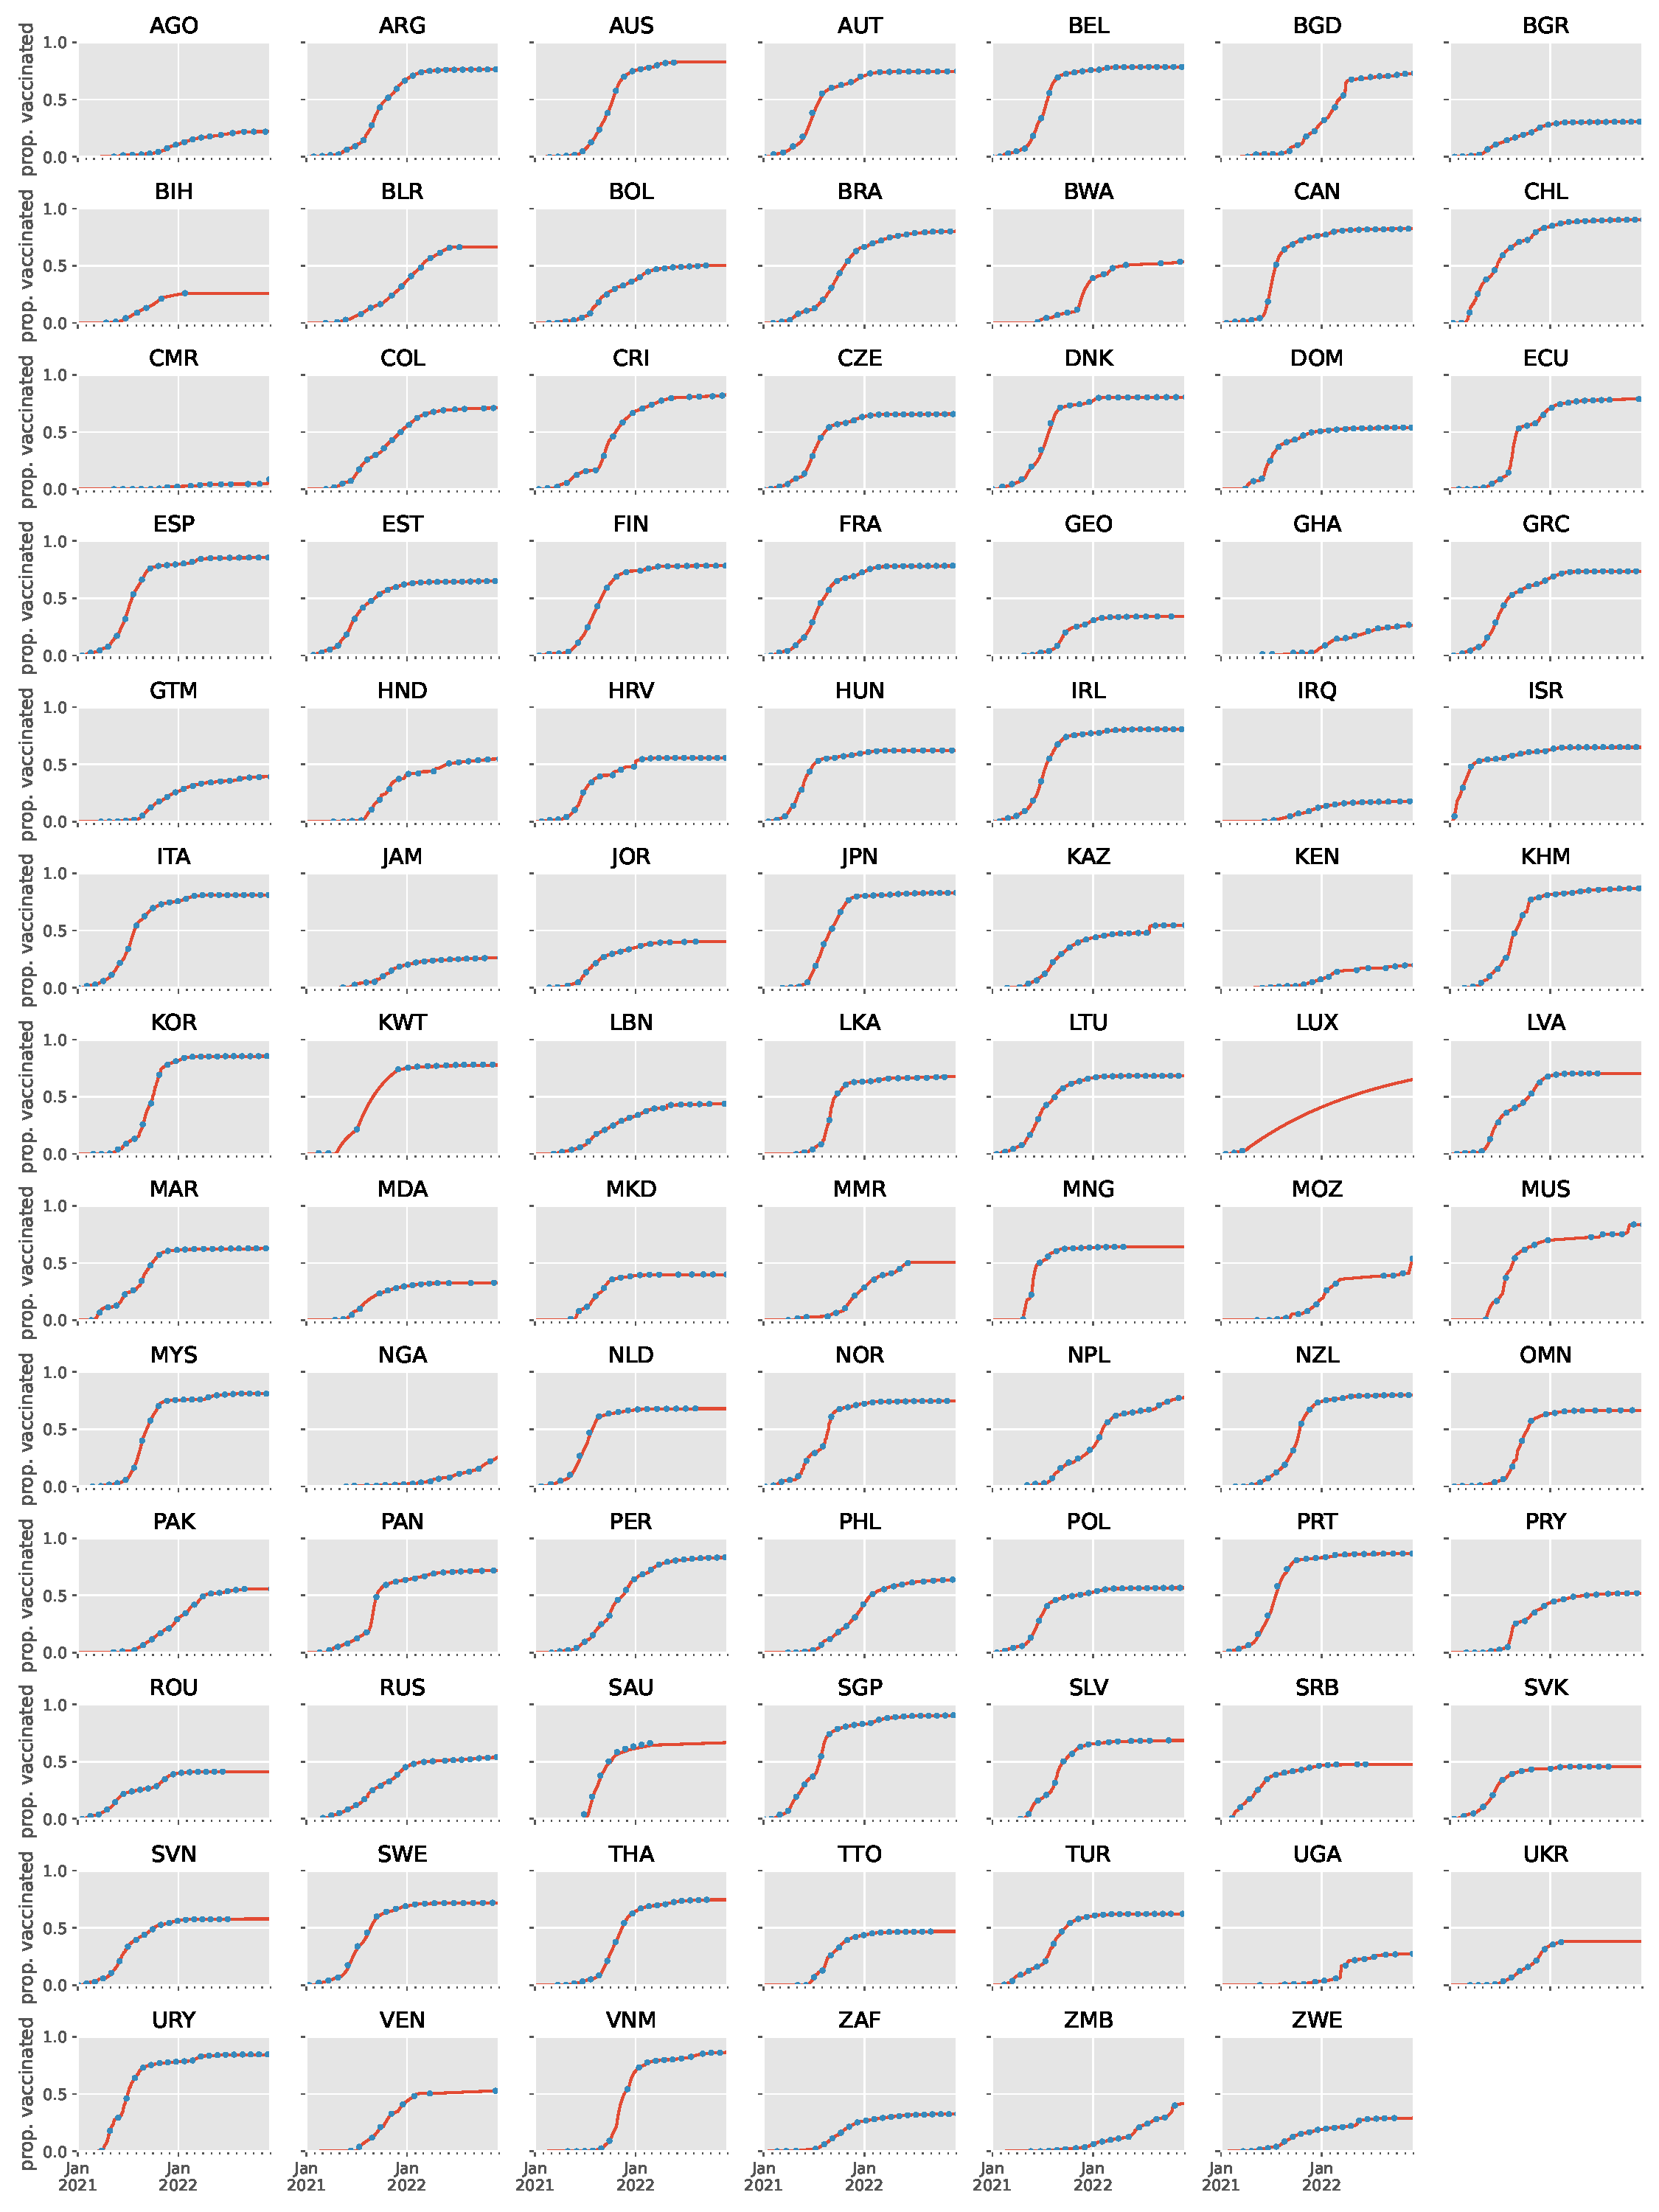
\includegraphics[width=1.0\textwidth]{../../tex_descriptions/projects/sm_covid/vacc_coverage.pdf}
    \end{center}
    \caption{Modelled vaccine coverage (lines) against data (dots).
    } 
    \label{fig:vaccination}
\end{figure}

The effect of vaccination on transmission is to partially reduce the rate of infection for all persons at-risk of infection in the vaccinated stratum.
This includes both fully susceptible (never previously infected) persons,
as well as recovered persons who are at risk of reinfection. The model allows for hybrid immunity
in the sense that the vaccination-induced relative reduction of transmission risk is multiplied with that induced by previous infection. Vaccination is also assumed to reduce the risk of hospitalisation and death 

Emerging variants of concern (VoCs) may partially escape vaccine-induced (as well as infection-induced) immunity, as described further below (\textcolor{red}{see Section / Table XX}).

